\documentclass[../Paper.tex]{subfiles}

\begin{document}
\section{Trajectory Optimization Model}

\subsection{Establishment of optimal model}

\subsubsection{Description}

In the previous section we have demonstrated the feasibility of launching solar sail spacecraft from earth to Mars orbit. In comparing the previous figures, we can find the attitude angle $\alpha$ and the surface of the solar sail A have certain influence on the trajectory of spacecraft. Thought understanding the differential equation \eqref{eq:diffx} \eqref{eq:diffy} the transit time t is determined by the attitude angle $\alpha$ and the surface of the solar sail A. So this section is in order to find the optimal solution, to decrease the transit time and insure the payload, to maximize the advantage of solar sails.

\subsubsection{Conditions of Capture by Mars}
% 分析由于火星引力捕获的作用,飞行器到达火星轨道的位置的讨论分析{}
According to actual condition, when the spacecraft near Mars, the influence of the Martian gravity is bigger and bigger, so we set up a Martian gravity range. When the spacecraft into the scope, we ignore the role of the sun's gravity, and the Martian gravity plays a leading role. In other words, the spacecraft was captured by Mars.  At this time, if the speed constraint is under certain conditions, it can land safely, so we can get the spacecraft to be captured by Mars as one of the constraints.

We suppose that when $ \dfrac{G_M}{G} = \varepsilon $ the spacecraft will be captured by Mars, according to the gravitational equation:
\begin{equation*}
\frac{G M_{M} m}{(r_{range})^2} = \frac{GM_{S}m}{ (R_{M}-r_{range})^2} \cdot \varepsilon
\end{equation*}
So here we get the distance constrain:
%因此这个地方得到距离约束条件:
\begin{equation*}
\varepsilon \cdot r_{range}^2 + 2\cdot R_{E} \cdot \dfrac{M_{M}}{M_{S}} r_{range} - R_{E}^2 \cdot \dfrac{M_{M}}{M_{S}} = 0
\end{equation*}

E.g. we suppose that $\varepsilon = 10$ after calculating we get the range of gravitational influence of Mars 
is $2.68 \times 10^{7} $. So in the constraint condition we set this  order of magnitude $(10^7)$ is reasonable.

\subsubsection{Mathematical formulation}
% 优化模型:目标函数:t;决策变量: alpha 和 A
As discussion above, we can take the below mathematical formulation of optimization model

\begin{dingautolist}{202}

\item \textbf{Objective function: $ \min{t = t(\alpha,A)} $ }

\item \textbf{Decision variable: $ \alpha , A $ }  
% t(A,alpha) 满足微分方程组

\item \textbf{$t(\alpha,A)$ satisfy system of differential equations \eqref{eq:diffx} \eqref{eq:diffy} }

\begin{equation*}
\vec{F_x} = (-\frac{GMmx}{(\sqrt{x^2+y^2})^3} + \dfrac{C_{1} A cos^2 \alpha}{\sqrt{x^2+y^2}} (cos\alpha\frac{x}{\sqrt{x^2+y^2}} - sin\alpha\frac{y}{\sqrt{x^2+y^2}}))\vec{u_x}
\end{equation*}

\begin{equation*}
\vec{F_y} = (-\frac{GMmy}{(\sqrt{x^2+y^2})^3} + \dfrac{C_{1} A cos^2 \alpha}{\sqrt{x^2+y^2}} (cos\alpha\frac{y}{\sqrt{x^2+y^2}} + sin\alpha\frac{x}{\sqrt{x^2+y^2}}))\vec{u_y}
\end{equation*}

\item \textbf{Constraint conditions:}
% 约束条件:4个初始条件 + 3个终止条件(1个用来提取其到达时间,另外两个用来判断其到达点是否满足条件),A有一个条件,alpha > 0

\begin{itemize}
	\item 

4 Initial conditions:
\begin{equation*}
\left\{\begin{array}{ll}
~& x(t=0) = R_{E}\\[2mm]
~& y(t=0) = 0 \\[2mm]
~& v_{x}(t=0) = 0 \\[2mm]
~& v_{y}(t=0) = V_{E}(Earth~revolution~speed) 
\end{array}\right.
\end{equation*}

\item 
4 End conditions:
\begin{equation*}
\left\{\begin{array}{ll}
~& x(t=t_{arrive})^2 + y(t=t_{arrive})^2 = R_{M}^2\\[2mm]
~& v_{x}(t=t_{arrive})^2 + v_{y}(t=t_{arrive})^2 \leq 9000 m \cdot s^{-1} \\[2mm]
~& x(t=t_{arrive}) = R_{M} \cos{ \left[ \dfrac{t_{arrive}}{T_{M}} \cdot 2\pi \right] } \\[2mm]
~& y(t=t_{arrive}) = R_{M} \sin{ \left[ \dfrac{t_{arrive}}{T_{M}} \cdot 2\pi \right] }
\end{array}\right.
\end{equation*}

Where the last 2 equations mean: when the solar sail get to Mars, time spent is $ t_{arrive} $,
at the end of this time, the position of Mars are  
$ \left( R_{M} \cos{ \left[ \dfrac{t_{arrive}}{T_{M}} \cdot 2\pi \right] } ,
 R_{M} \sin{ \left[ \dfrac{t_{arrive}}{T_{M}} \cdot 2\pi \right] } \right) $, 
where $ T_{M} $ is the period of revolution of Mars, the position of solar sail $( x(t=t_{arrive}) , y(t=t_{arrive}) )$ 
should meet this point.

\item 
2 conditions of range of decision conditions:
$$ 0 < A < \dfrac{m}{\sigma} = 285714m^2 $$
$$ 0 < \alpha < \dfrac{\pi}{2} $$
\end{itemize}

\end{dingautolist}

\subsection{Realization by program}
% 程序实现,通过迭代,A 在外层, alpha 在内层进行循环迭代求解,得出符合条件的一组值(A,alpha), 再从里面挑选 t 最小点


\textbf{STEP0} : Start;\\[1mm]

\textbf{STEP1} : Input kinematical differential equations \eqref{eq:diffx} \eqref{eq:diffy} and initial conditions;\\[1mm]

\textbf{STEP2} : Give the range of the surface A and the attitude angle $\alpha$;\\[1mm]

\textbf{STEP3} : Set the step length of A and $\alpha$, start to loop;\\[1mm]

\textbf{STEP4} : Judge the solution : the relative speed between Mars and the spacecraft is less 
than $9km/s$, the distance between Mars and the spacecraft is less than $r_{range}$;\\[1mm]

\textbf{STEP5} : Output the (A,$\alpha$) that meet the judgement;\\[1mm]

The detailed program code will be pasted to Appendix.

\subsection{Result}
% 数值结果和结果图片展示

After the iterative process by Matlab , luckily we seek 7 optimal values that satisfy all constraint conditions.
By the program, we also obtain the transit time(time when the solar sailing arrive the destination) 
$ t_{arrive} $ and the effective load(the total mass removes the quality of the solar sail) $ m_{e} $, and
$$ m_{e} = m - \sigma \cdot A $$
where $A$ is the area of solar sail, $ \sigma = 7g\cdot m^{-2} $ is the density of solar sail and 
$ m = 2000kg $ is the total mass of solar sail and effective load $m_{e}$. 

Next is the table of 7 optimal values found by program and we list the corrosponding values of $A$, $t_{arrive}$ and $m_{e}$.

\renewcommand\arraystretch{2} % <-- 设置表格行高
\begin{table}[H]
\centering
\scriptsize %此处写字体大小控制命令
\begin{tabular}{ p{1.5cm}<{\centering}|p{1.5cm}<{\centering}|p{1.5cm}<{\centering}|p{1.5cm}<{\centering}|
				 p{1.5cm}<{\centering}|p{1.5cm}<{\centering}|p{1.5cm}<{\centering}|p{1.5cm}<{\centering}  }
\hline
  &  1  &  2  &  3  &  4  &  5   &  6  &  7 \\
\hline
$ \alpha(rad) $ & 0.21195 & 0.2198 & 0.14915 & 0.1099 & 0.1256 & 0.0658 & 0.0942 \\
\hline
$ \sqrt{A}(m) $ & 420 & 420 & 440 & 460 & 460 & 480 & 480 \\
\hline
$ A(m^2) $ & 176400 & 176400 & 193600 & 211600 & 211600 & 230400 & 230400 \\
\hline
$ t_{arrive}(day)  $ & 765 & 770 & 548 & 525 & 564 & 483 & 840 \\
\hline
$ m_{e}(kg) $ & 765.2 & 765.2 & 644.8 & 518.8 & 518.8 & 387.2 & 387.2 \\
\hline
\end{tabular}
\caption{List of 7 optimal values}
\label{Tableofoptimalvalues}
\end{table}  

By this table, we can find the minimum transit time $t_{arrive}$ is 483 days, the corrosponding 
effective load is 387.2 kg account for 19.36$\%$ of the total mass. If we want to get the 
maximum effective load $m_{e}$, we need about 770 days.

Next are specific trajectories of the 7 cases above.

\begin{figure}[H]
 \begin{minipage}[t]{0.5\linewidth}
 \centering{}
 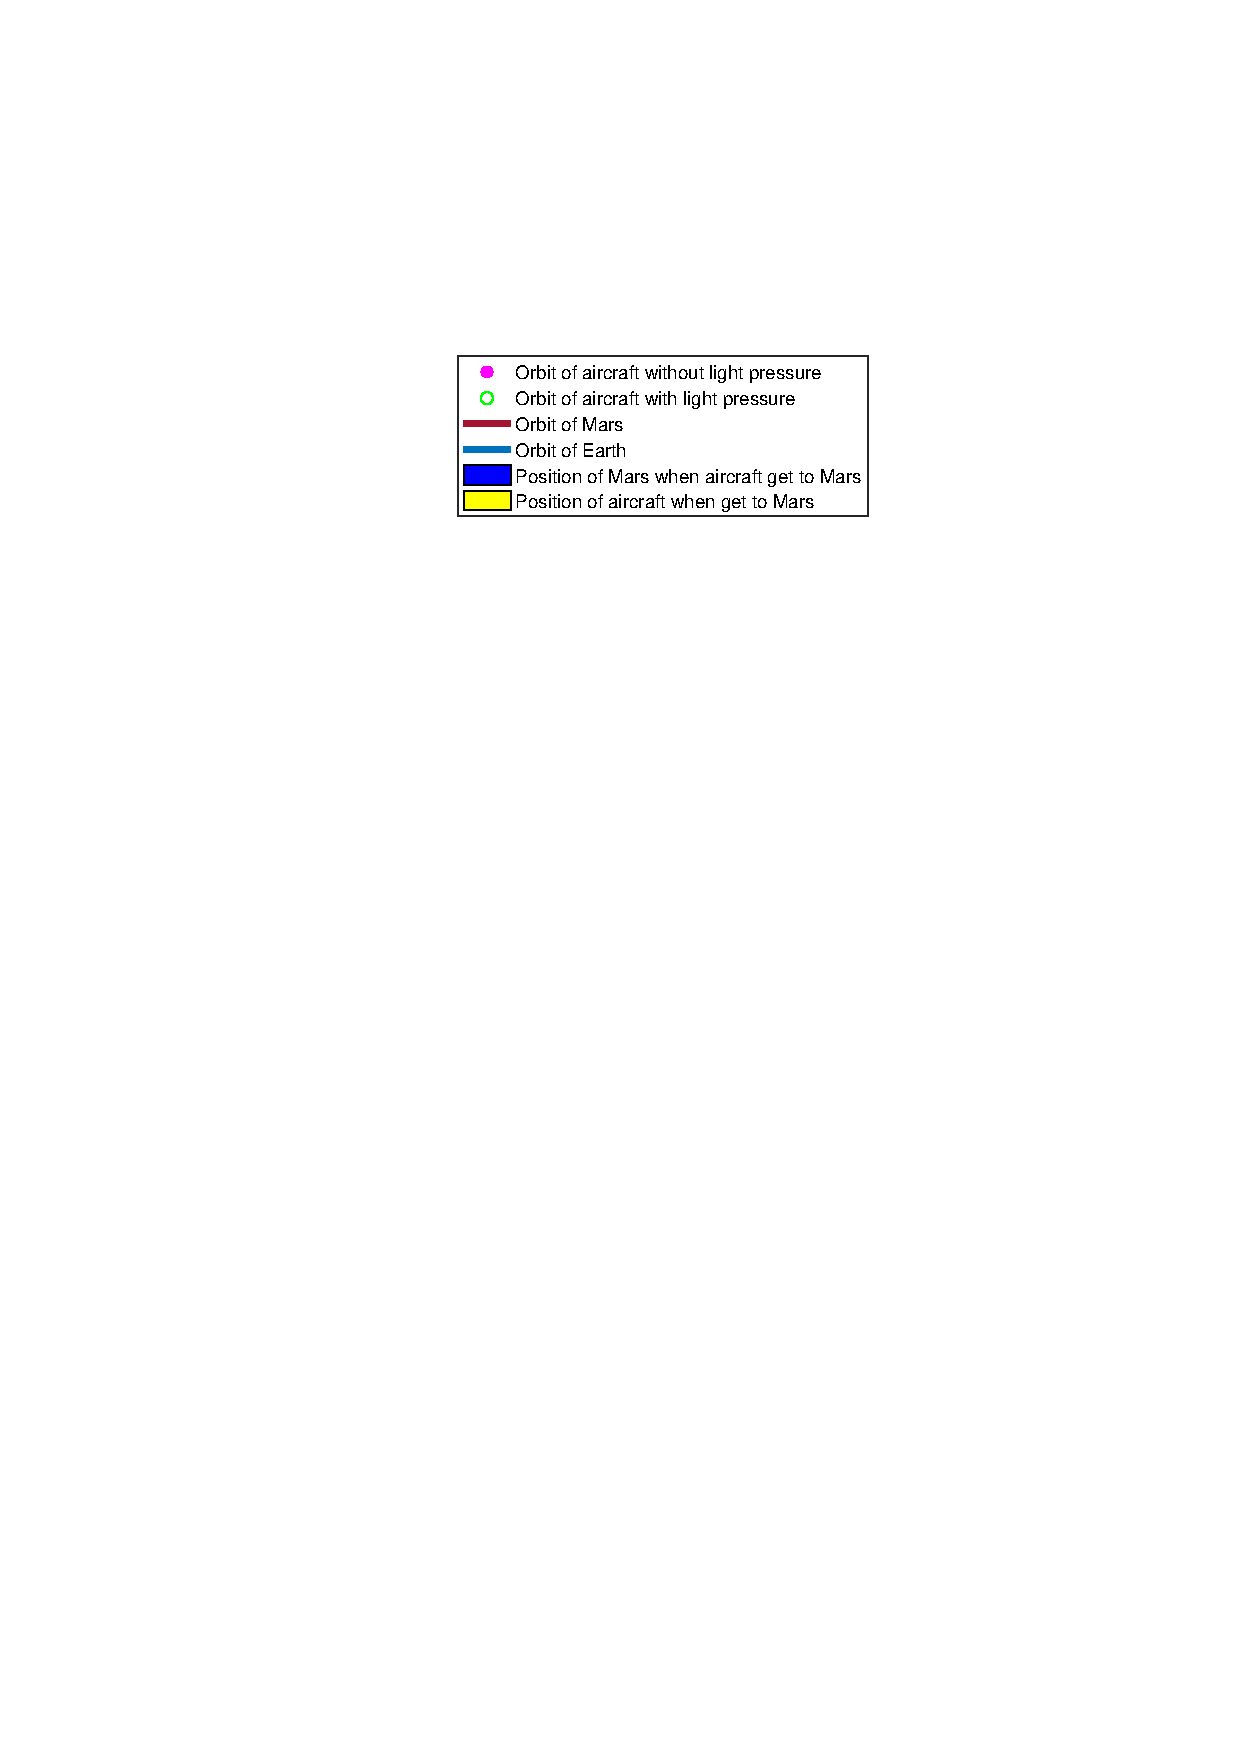
\includegraphics[width=7cm]{../Figures/label_of_7_orbits.pdf}
 \label{fig:orbitlegend}
 \caption{Legend of lines and points in figures below}
 \end{minipage}
 \begin{minipage}[t]{0.5\linewidth}
 \centering{}
 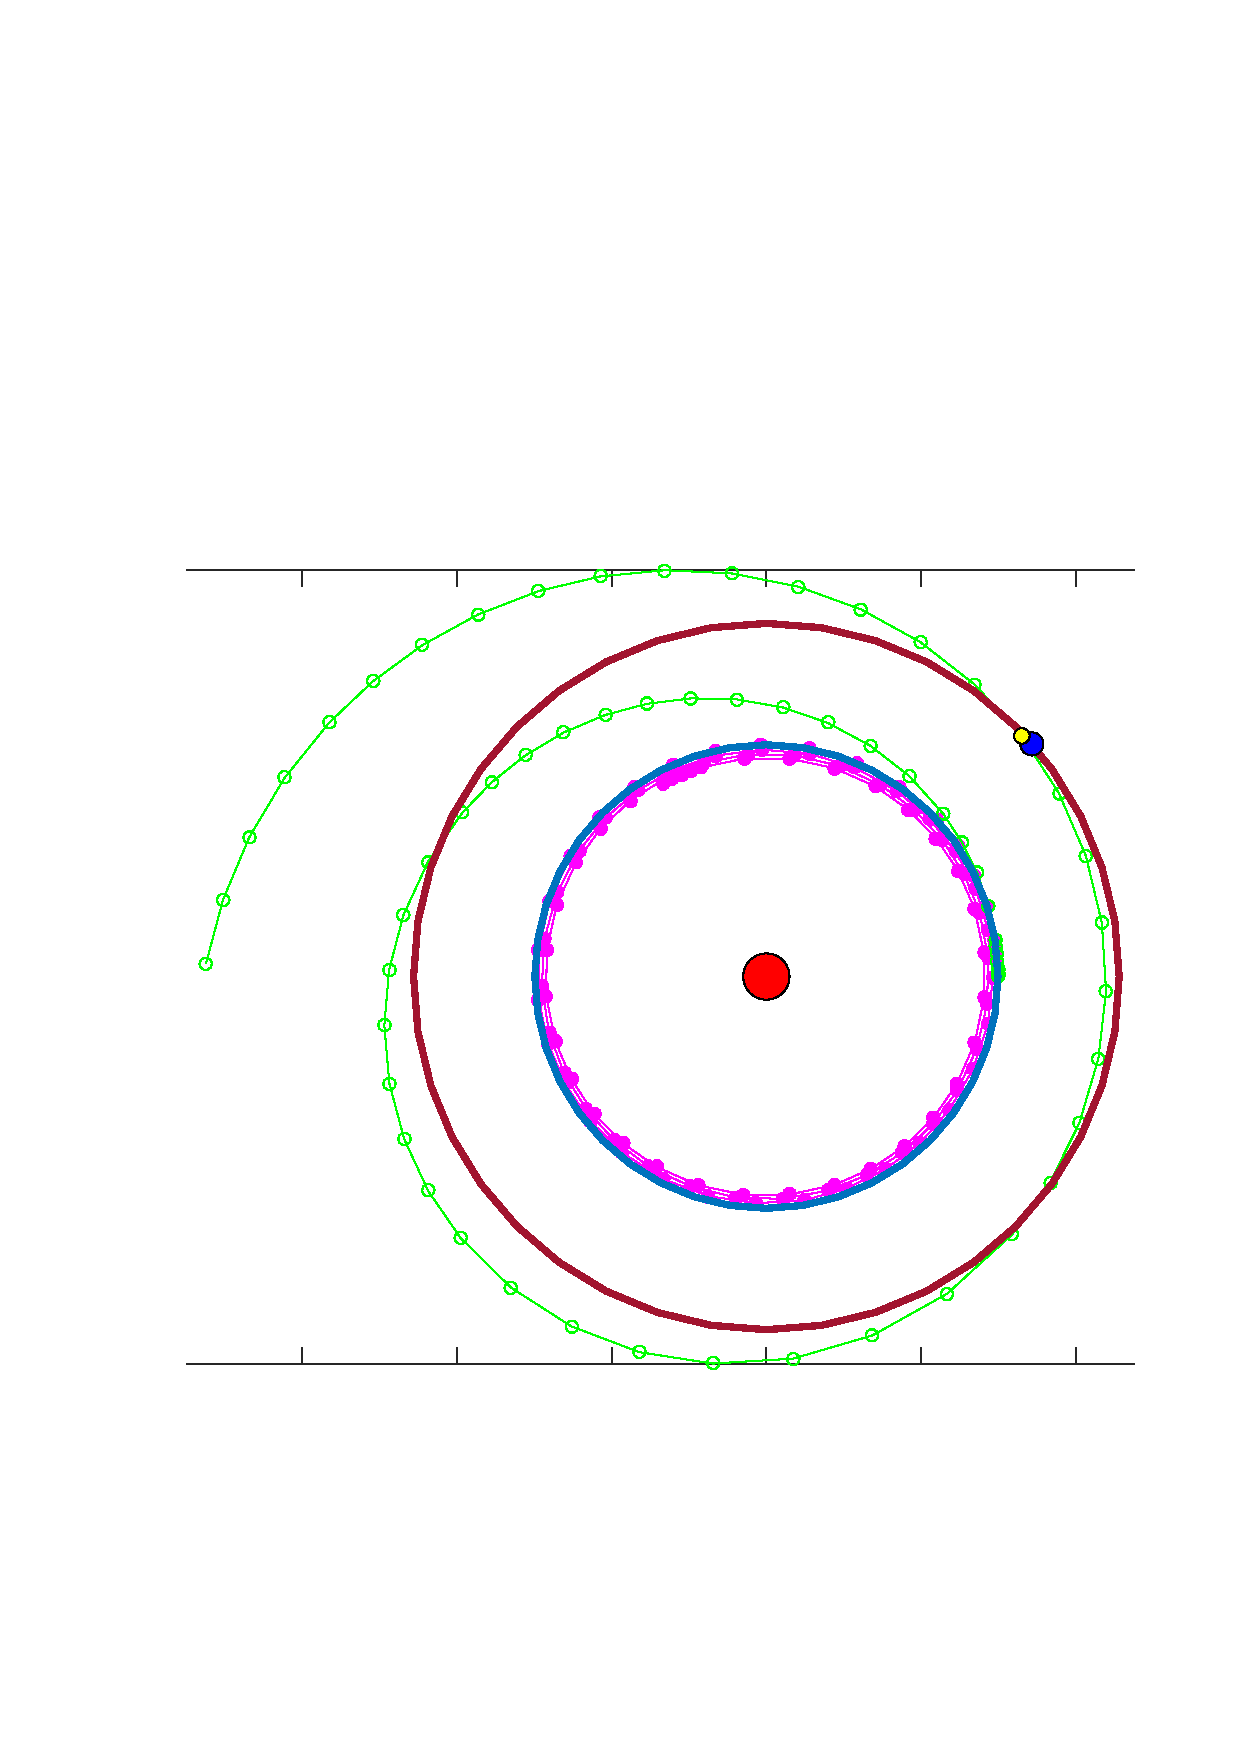
\includegraphics[width=7cm]{../Figures/orbit1.pdf}
 \label{fig:orbit1}
\caption{$alpha=0.21195$,$A=176400$}
 \end{minipage}
\end{figure}
\begin{figure}[H]
 \begin{minipage}[t]{0.5\linewidth}
 \centering{}
 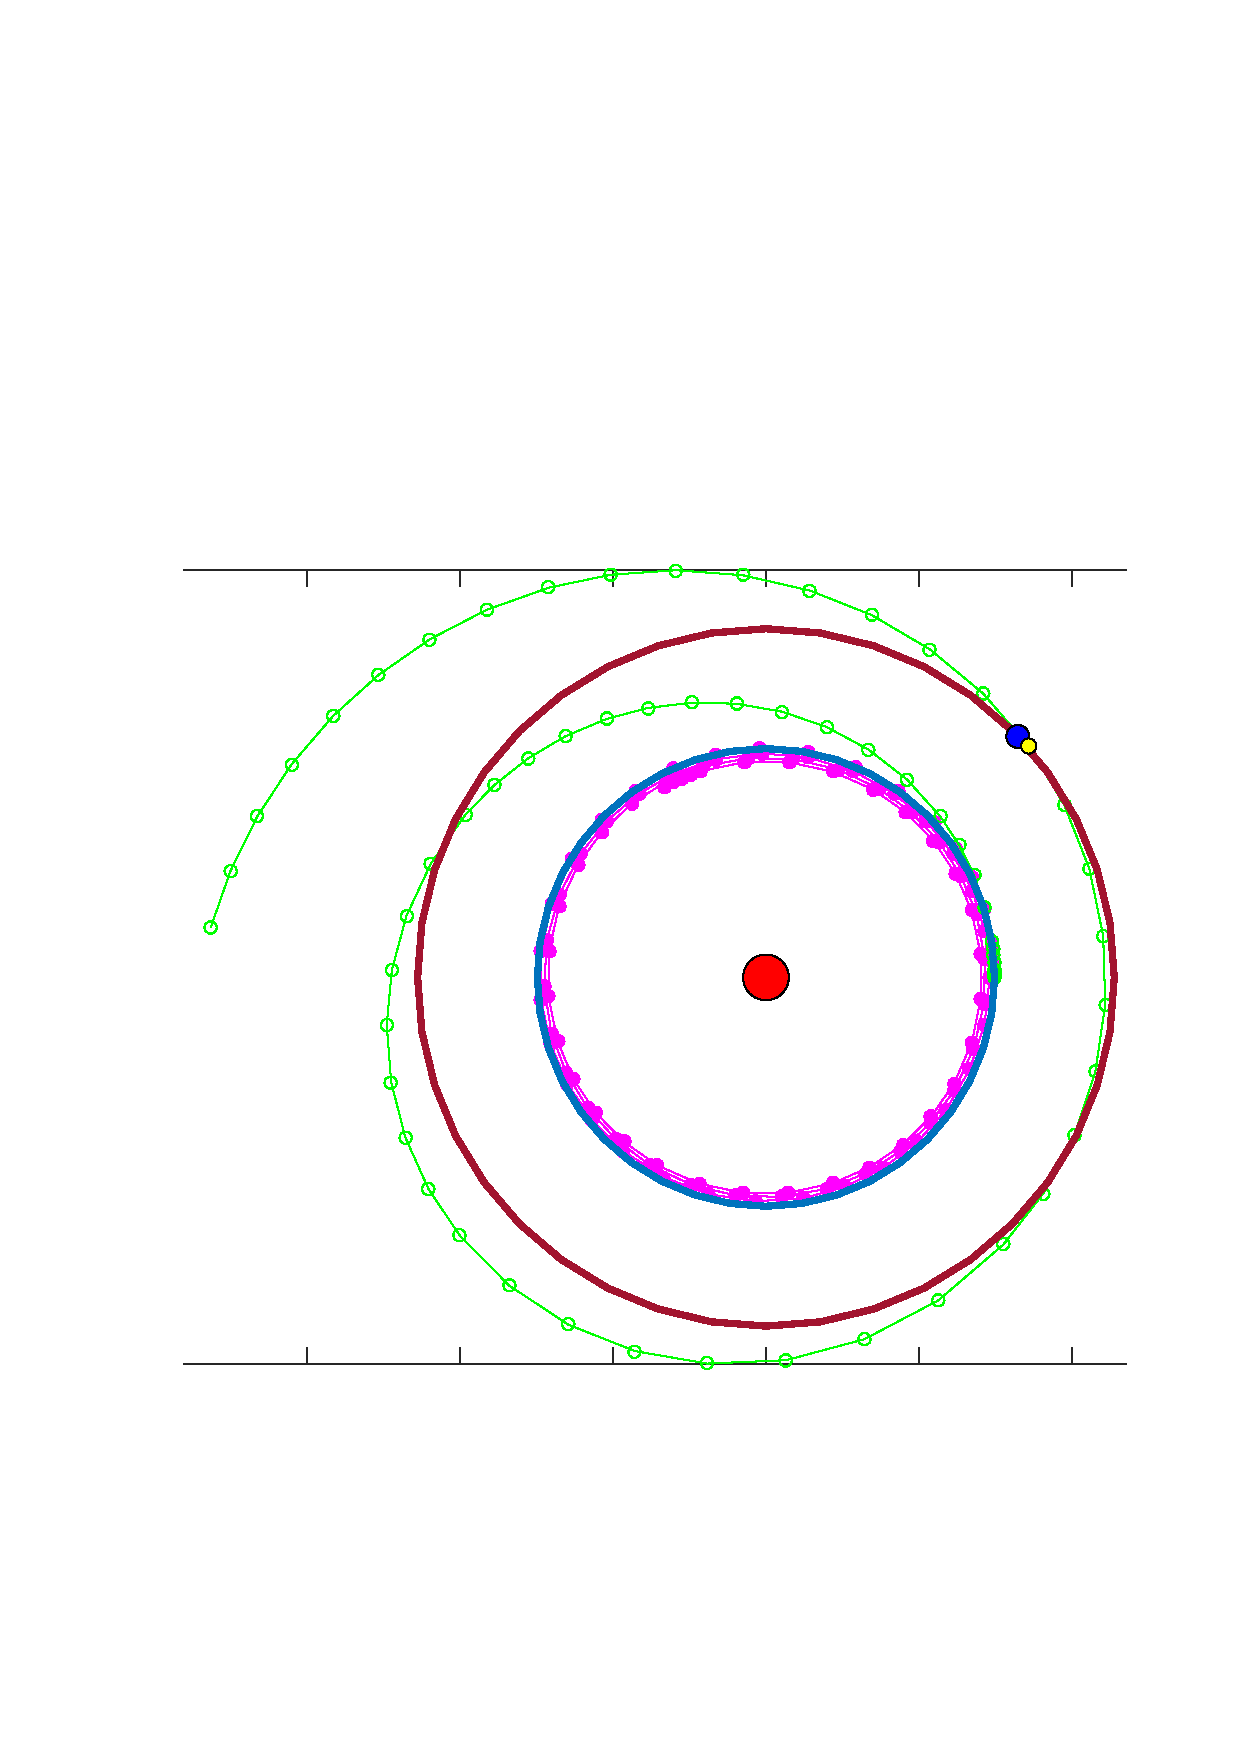
\includegraphics[width=7cm]{../Figures/orbit2.pdf}
 \label{fig:orbit2}
\caption{$alpha=0.2198$,$A=176400$}
 \end{minipage}
 \begin{minipage}[t]{0.5\linewidth}
 \centering{}
 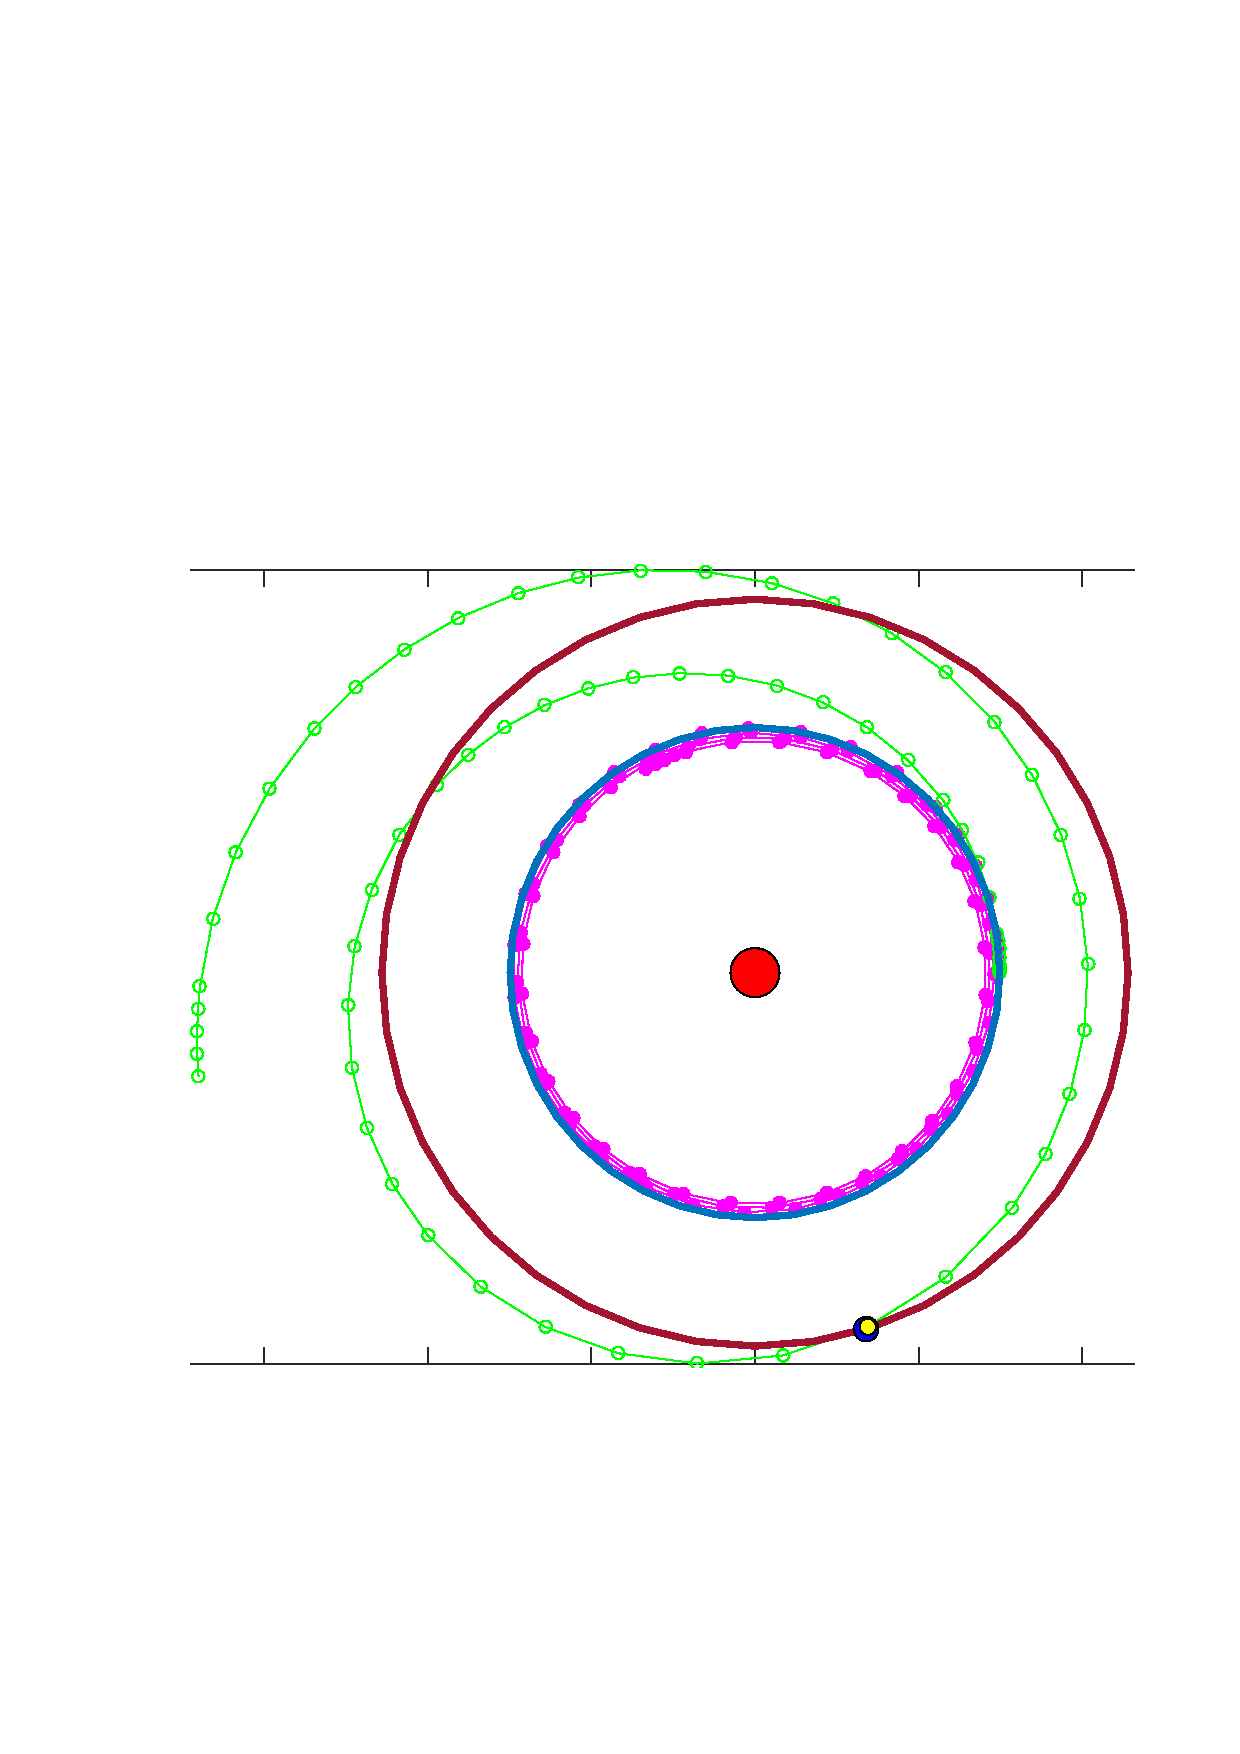
\includegraphics[width=7cm]{../Figures/orbit3.pdf}
 \label{fig:orbit3}
\caption{$alpha=0.14915$,$A=193600$}
 \end{minipage}
\end{figure}
\begin{figure}[H]
 \begin{minipage}[t]{0.5\linewidth}
 \centering{}
 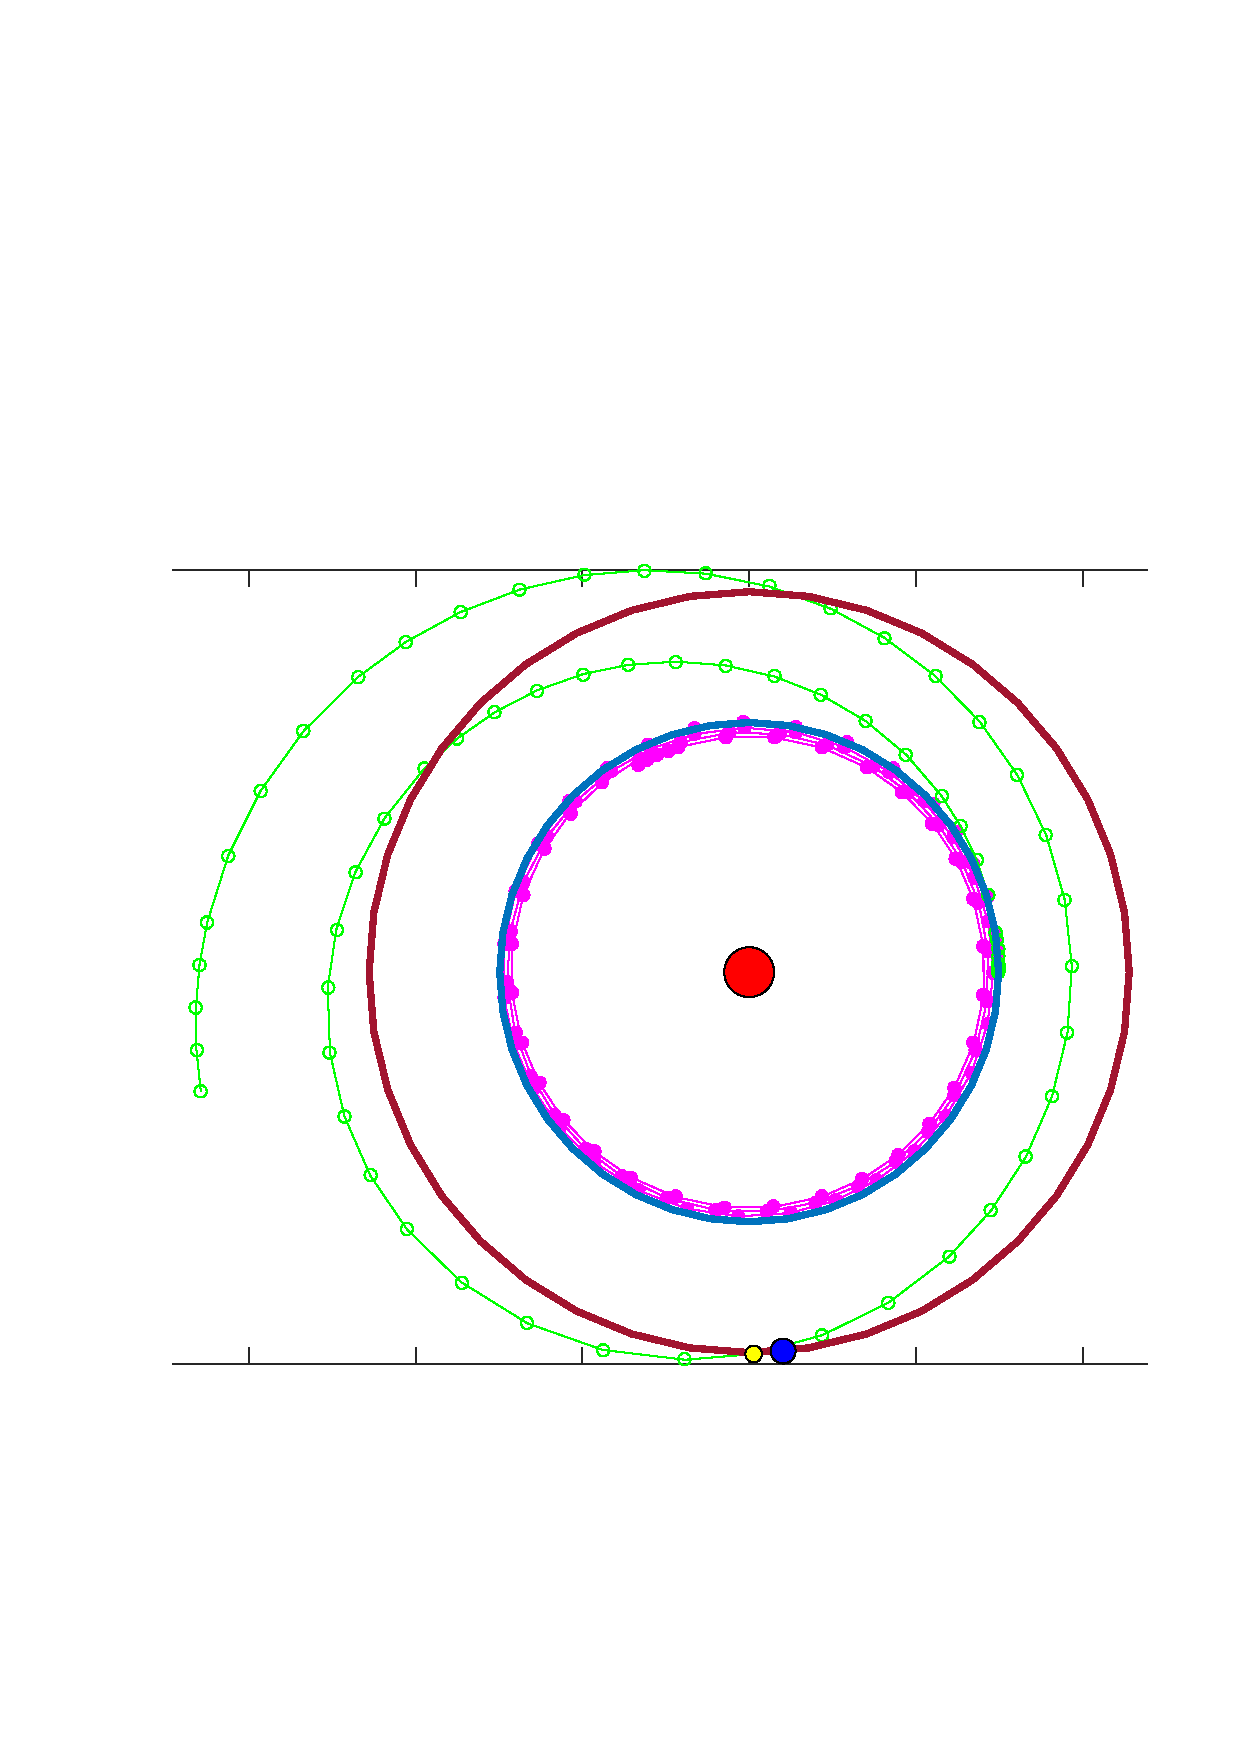
\includegraphics[width=7cm]{../Figures/orbit4.pdf}
 \label{fig:orbit4}
\caption{$alpha=0.1099$,$A=211600$}
 \end{minipage}
 \begin{minipage}[t]{0.5\linewidth}
 \centering{}
 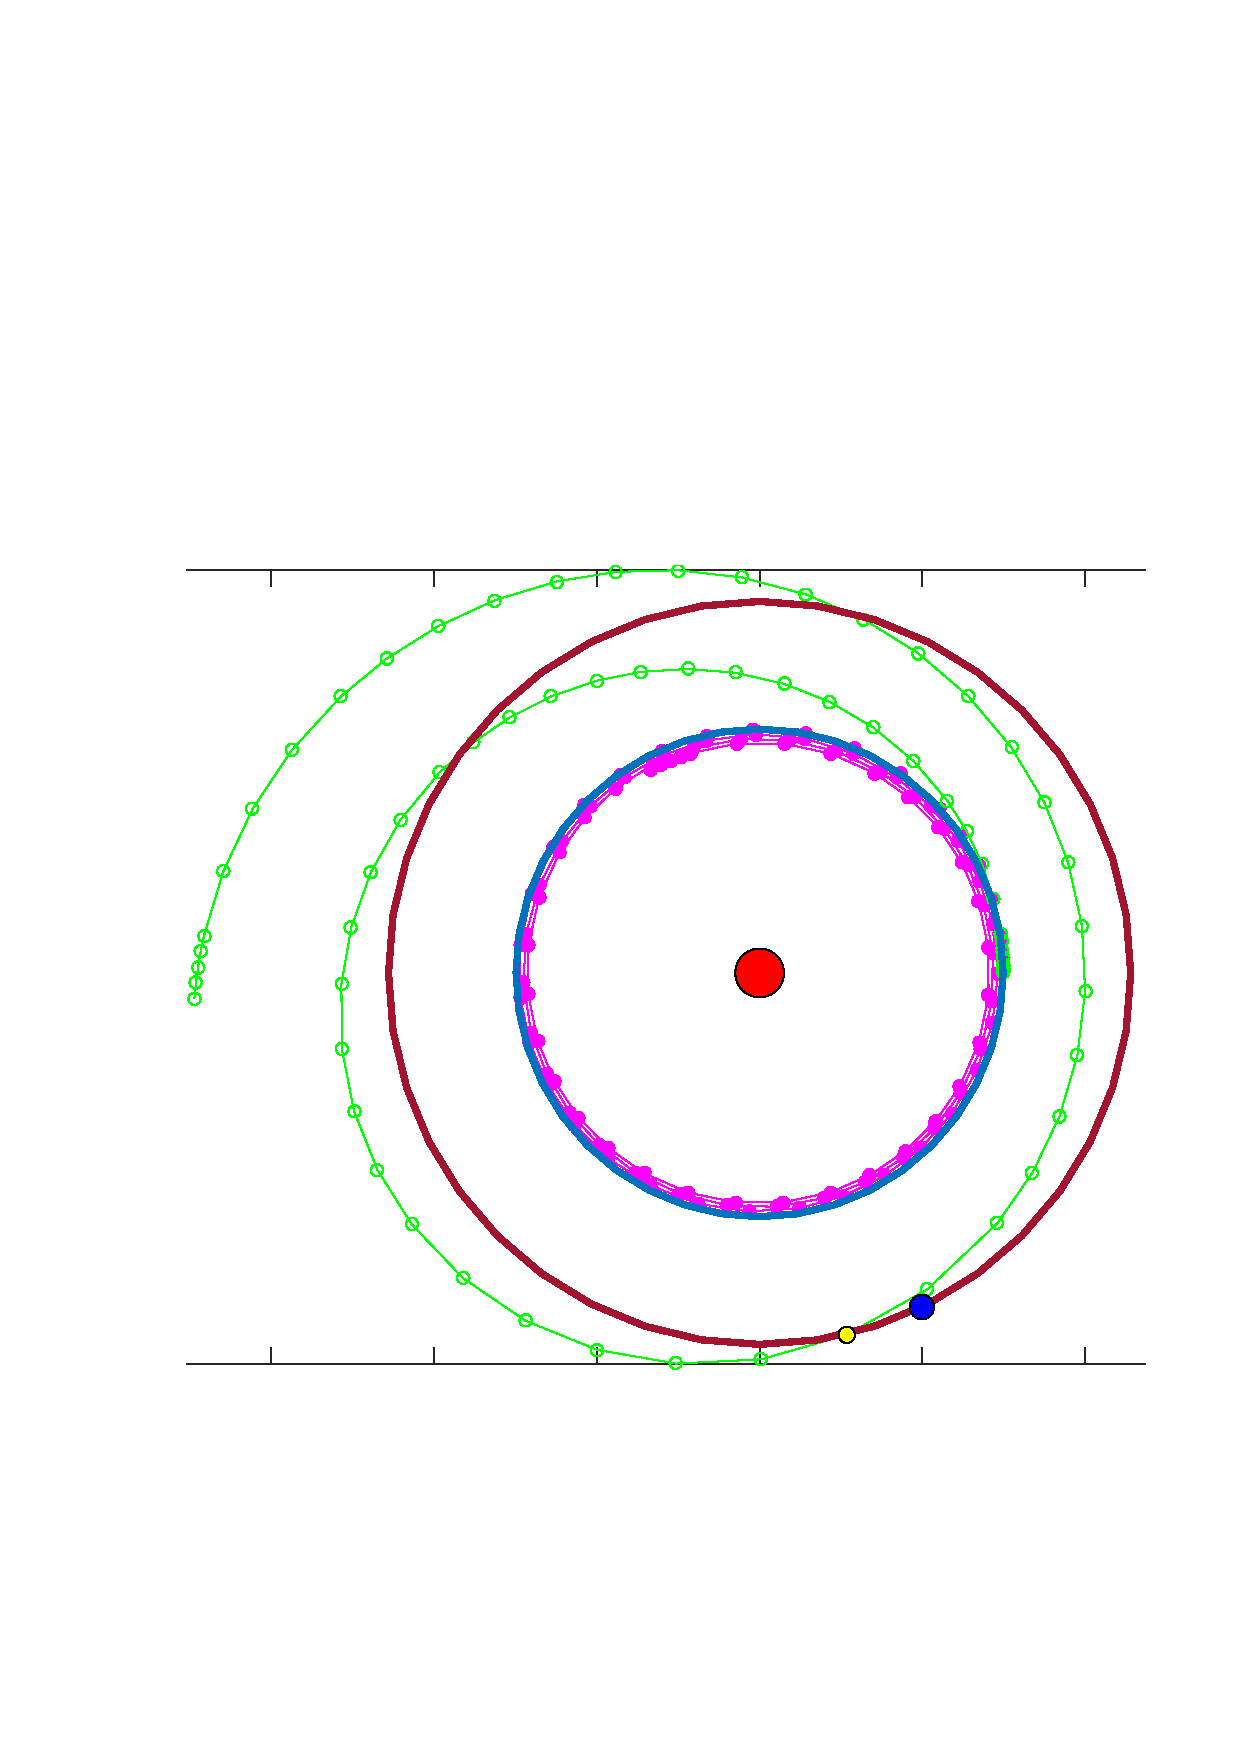
\includegraphics[width=7cm]{../Figures/orbit5.pdf}
 \label{fig:orbit5}
\caption{$alpha=0.1256$,$A=211600$}
 \end{minipage}
\end{figure}
\begin{figure}[H]
 \begin{minipage}[t]{0.5\linewidth}
 \centering{}
 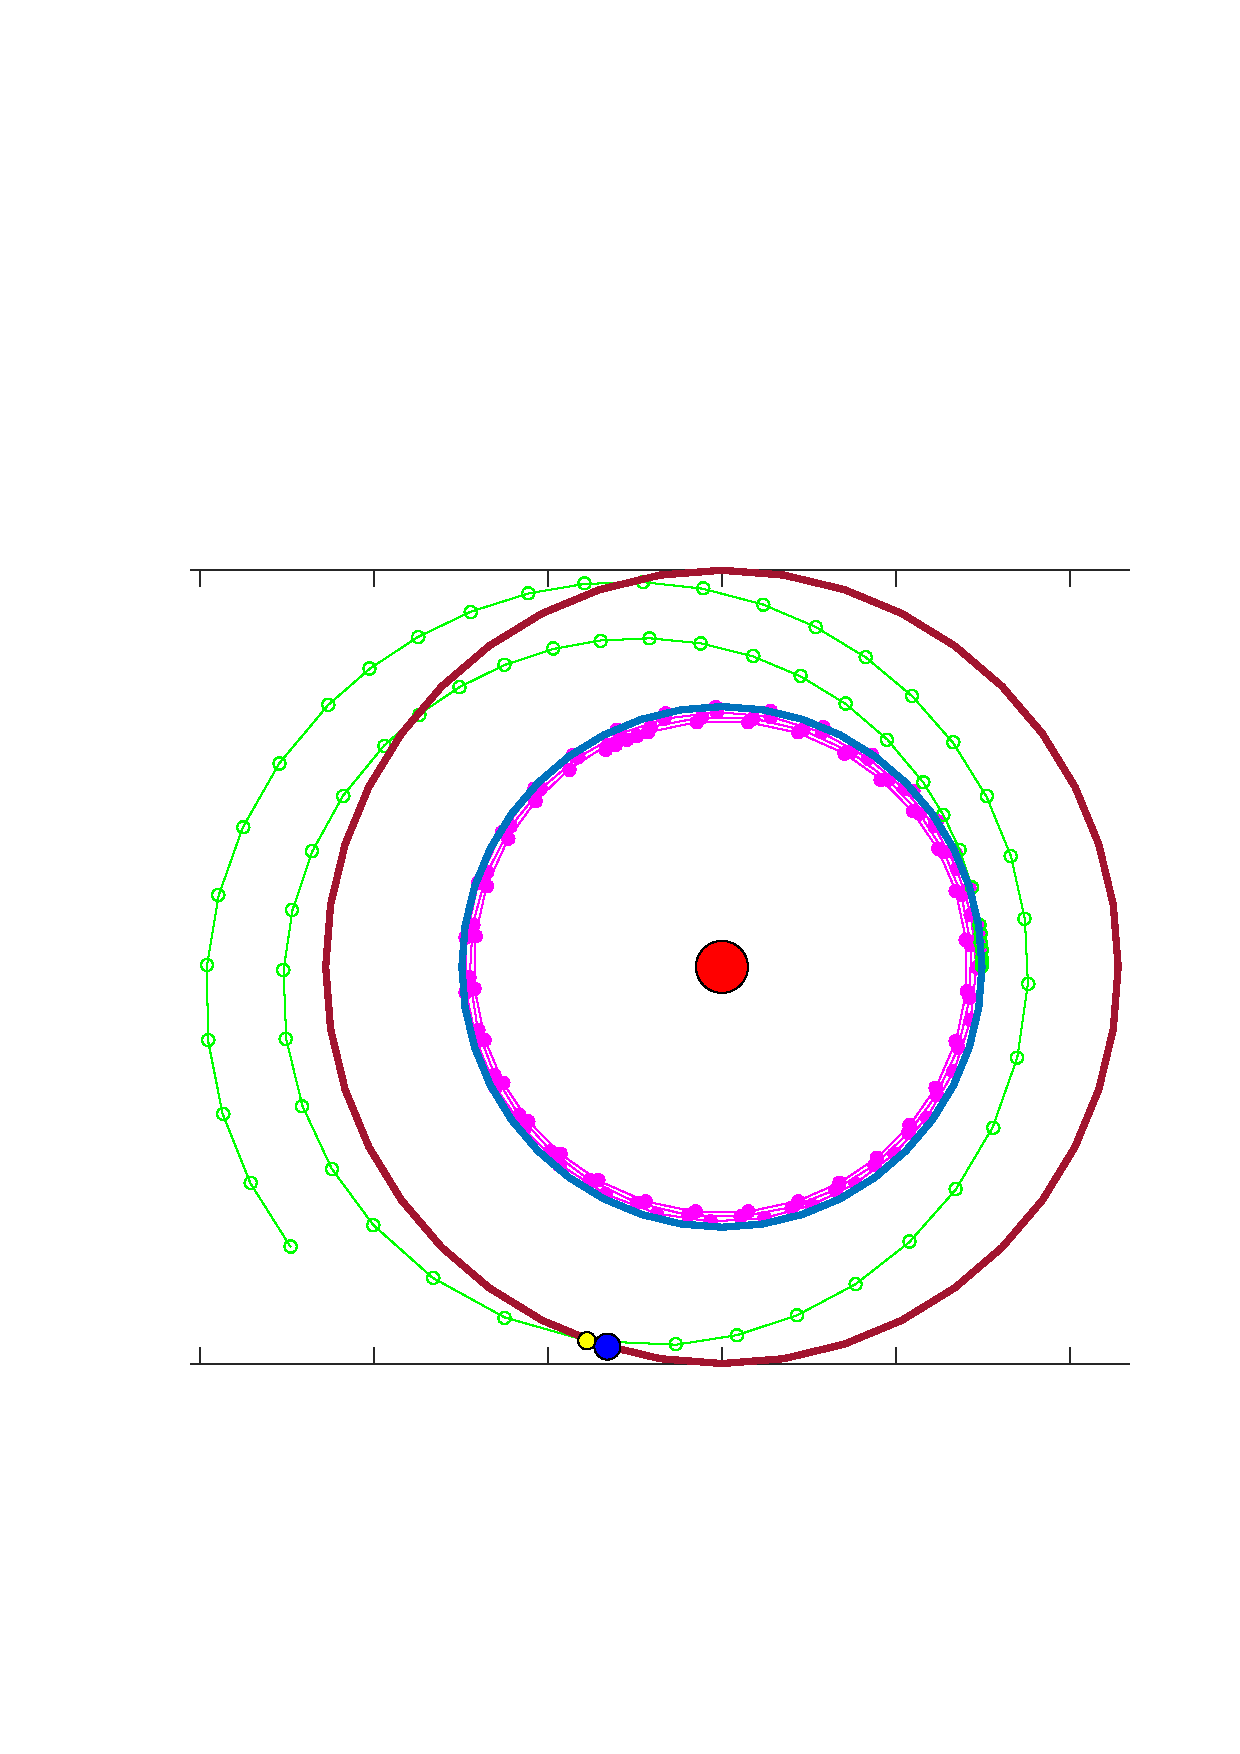
\includegraphics[width=7cm]{../Figures/orbit6.pdf}
 \label{fig:orbit6}
\caption{$alpha=0.0658$,$A=230400$}
 \end{minipage}
 \begin{minipage}[t]{0.5\linewidth}
 \centering{}
 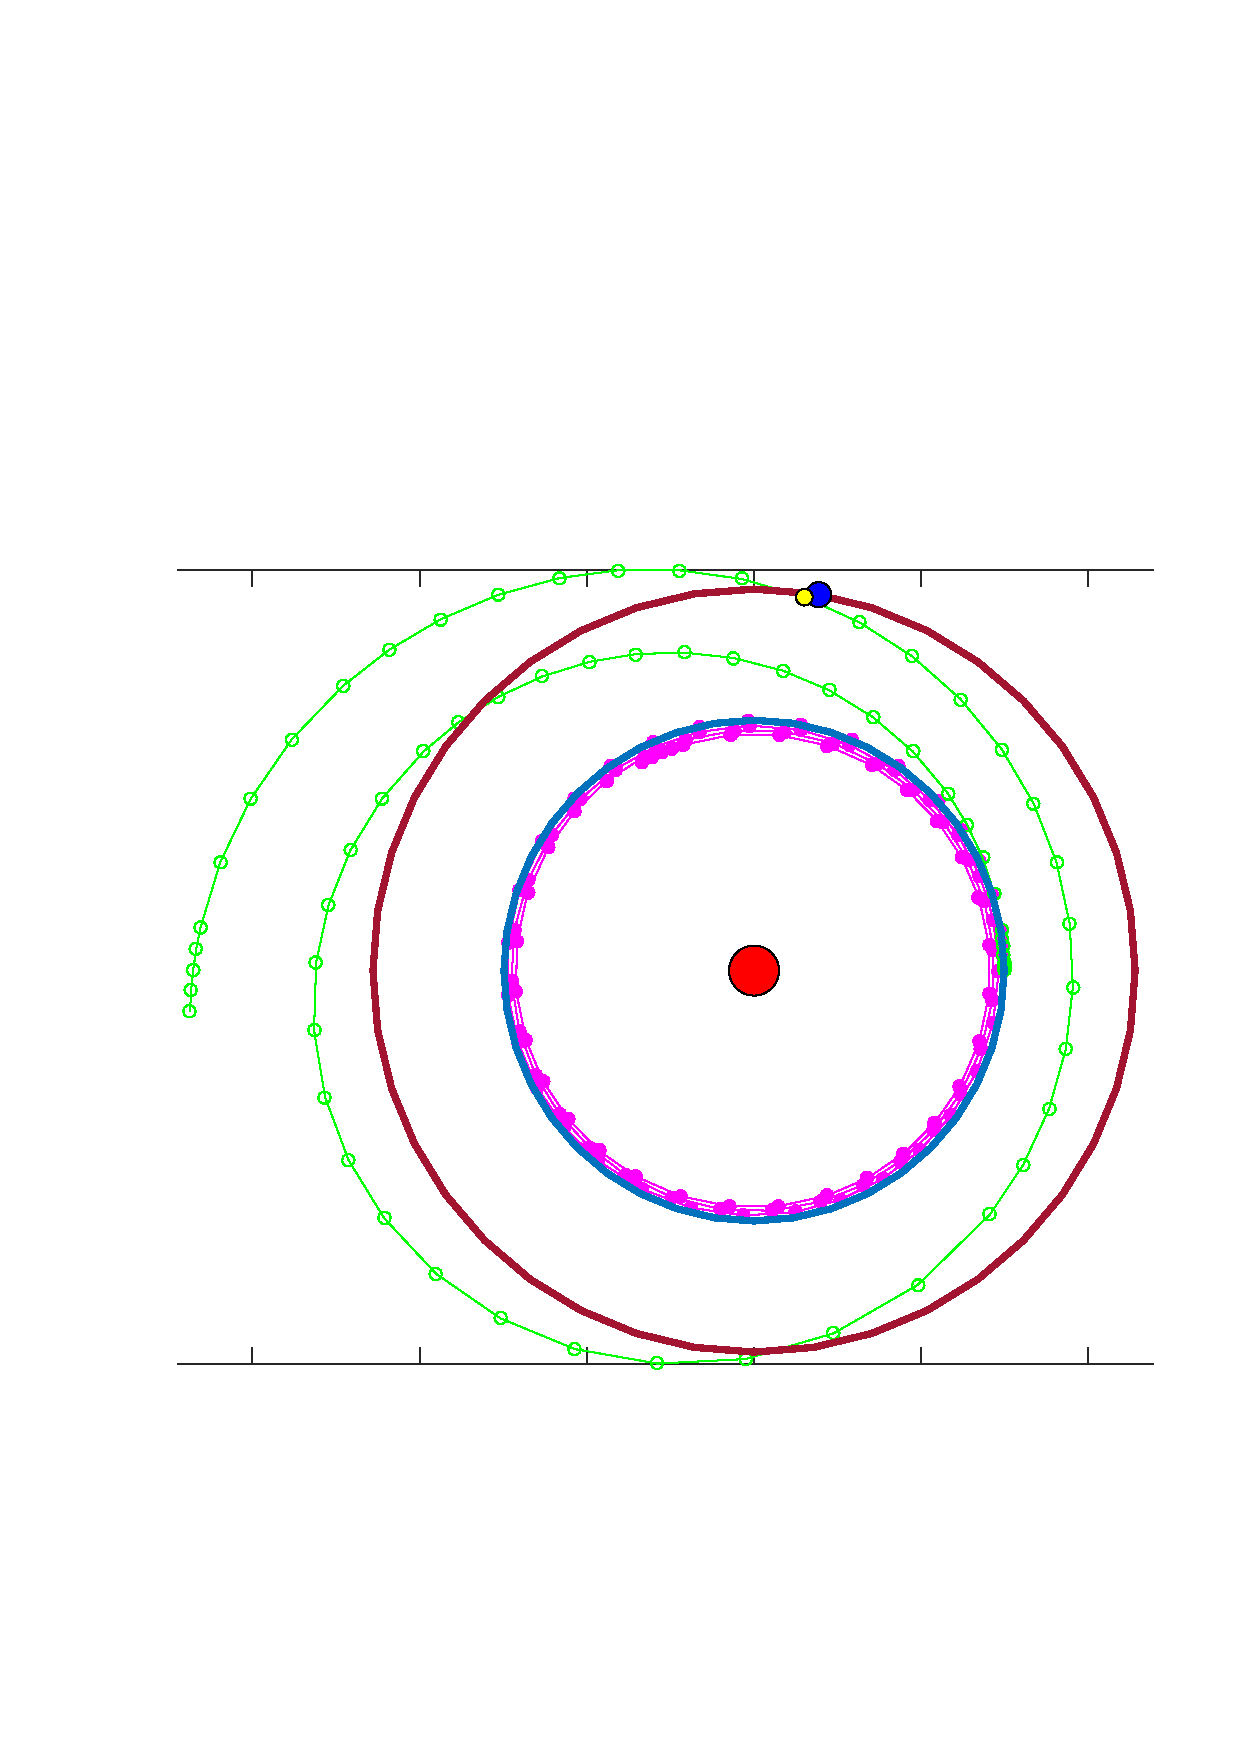
\includegraphics[width=7cm]{../Figures/orbit7.pdf}
 % \caption{spiralling outward($F_P\cdot\alpha<0$)}
 \label{fig:orbit7}
\caption{$alpha=0.0942$,$A=230400$}
 \end{minipage}
\end{figure}

\end{document}